%%%%%%%%%%%%%%%%%%%%%%%%%%%%%%%%%%%%%%%%%%%%%%%%%%%%%%%%%%%%%%%%%%%%%%%%%%%%%%%%
%2345678901234567890123456789012345678901234567890123456789012345678901234567890
%        1         2         3         4         5         6         7         8

%\documentclass[journal,transmag]{IEEEtran}% Comment this line out if you need a4paper

\documentclass[10pt, conference]{ieeeconf}      % Use this line for a4 paper


\IEEEoverridecommandlockouts                              % This command is only needed if 
                                                          % you want to use the \thanks command

%\overrideIEEEmargins                                      % Needed to meet printer requirements.

% See the \addtolength command later in the file to balance the column lengths
% on the last page of the document

% The following packages can be found on http:\\www.ctan.org
%\usepackage{graphics} % for pdf, bitmapped graphics files
%\usepackage{epsfig} % for postscript graphics files
%\usepackage{mathptmx} % assumes new font selection scheme installed
%\usepackage{times} % assumes new font selection scheme installed
%\usepackage{amsmath} % assumes amsmath package installed
%\usepackage{amssymb}  % assumes amsmath package installed

\newtheorem{theorem}{Theorem}[section]
\newtheorem{lemma}[theorem]{Lemma}
\newtheorem{proposition}[theorem]{Proposition}
\newtheorem{corollary}[theorem]{Corollary}
\usepackage[ruled,vlined]{algorithm2e}
\usepackage{url}
\newenvironment{definition}[1][Definition]{\begin{trivlist}
\item[\hskip \labelsep {\bfseries #1}]}{\end{trivlist}}

\newcommand{\qed}{\nobreak \ifvmode \relax \else
      \ifdim\lastskip<1.5em \hskip-\lastskip
      \hskip1.5em plus0em minus0.5em \fi \nobreak
      \vrule height0.75em width0.5em depth0.25em\fi}

\def\lc{\left\lfloor}   
\def\rc{\right\rfloor}

\usepackage{amsmath,amssymb}

\usepackage{tabularx}
\usepackage{tikz,hyperref,graphicx,units}
\usepackage{subfigure}
\usepackage{benktools}
\usepackage{bbm}
\renewcommand{\baselinestretch}{.5}

\usepackage{caption}
\usepackage{epstopdf}
\renewcommand{\captionfont}{\footnotesize}
\usepackage{sidecap,wrapfig}
\usepackage[ruled,vlined]{algorithm2e}
\DeclareMathOperator*{\argmin}{arg\,min}
\DeclareMathOperator*{\argmax}{arg\,max}
\newcommand{\abs}[1]{\lvert#1\rvert} 
\newcommand{\norm}[1]{\lVert#1\rVert}
%\newcommand{\suchthat}{\mid}
\newcommand{\suchthat}{\ \big|\ }
\newcommand{\ba}{\mathbf{a}}
\newcommand{\bb}{\mathbf{b}}
\newcommand{\bc}{\mathbf{c}}
\newcommand{\bd}{\mathbf{d}}
\newcommand{\bg}{\mathbf{g}}
\newcommand{\bj}{\mathbf{j}}
\newcommand{\bn}{\mathbf{n}}
\newcommand{\bp}{\mathbf{p}}
\newcommand{\bw}{\mathbf{w}}
\newcommand{\bt}{\mathbf{t}}
\newcommand{\bu}{\mathbf{u}}
\newcommand{\by}{\mathbf{y}}
\newcommand{\bx}{\mathbf{x}}
\newcommand{\bz}{\mathbf{z}}
\newcommand{\bbf}{\mathbf{f}}
\newcommand{\bzero}{\mathbf{0}}
\newcommand{\bG}{\mathbf{G}}
\newcommand{\bA}{\mathbf{A}}
\newcommand{\bW}{\mathbf{W}}
\newcommand{\bX}{\mathbf{X}}
\newcommand{\mX}{\mathcal{X}}
\newcommand{\mD}{\mathcal{D}}
\newcommand{\mG}{\mathcal{G}}
\newcommand{\mN}{\mathcal{N}}
\newcommand{\mW}{\mathcal{W}}
\newcommand{\mF}{\mathcal{F}}
\newcommand{\bZ}{\mathbf{Z}}
\newcommand{\bbZ}{\mathbb{Z}}
\newcommand{\mR}{\mathcal{R}}

\newcommand{\bfc}{W}
\newcommand{\Qinf}{Q_{\infty}}
\newcommand{\st}[1]{_\text{#1}}
\newcommand{\rres}{r\st{res}}
\newcommand{\pos}[1]{(#1)^+}
\newcommand{\depth}{\operatorname{depth}}
\newcommand{\dist}{\operatorname{dist}}
\newcommand{\convhull}{\operatorname{ConvexHull}}
\newcommand{\minksum}{\operatorname{MinkowskiSum}}

\newcommand{\specialcell}[2][c]{ \begin{tabular}[#1]{@{}c@{}}#2\end{tabular}}
\newcommand{\acro}{SHIV}
\newcommand\independent{\protect\mathpalette{\protect\independenT}{\perp}}
\def\independenT#1#2{\mathrel{\rlap{$#1#2$}\mkern2mu{#1#2}}}

\newcolumntype{L}[1]{>{\RaggedRight\hspace{0pt}}p{#1}}
\newcolumntype{R}[1]{>{\RaggedLeft\hspace{0pt}}p{#1}}

%\newtheorem{lemma}{Lemma}[section]
%\newtheorem{theorem}{Theorem}[section]
\newtheorem{defn}{Definition}[section]

\newboolean{include-notes}
\setboolean{include-notes}{true}
\newcommand{\adnote}[1]{\ifthenelse{ \boolean{include-notes}}%
 {\textcolor{blue}{\textbf{AD: #1}}}{}}
 
 \newcommand{\sknote}[1]{\ifthenelse{ \boolean{include-notes}}%
 {\textcolor{blue}{\textbf{SK: #1}}}{}}
 
  \newcommand{\mlnote}[1]{\ifthenelse{ \boolean{include-notes}}%
 {\textcolor{purple}{\textbf{ML: #1}}}{}}
 
 \newcommand{\jmnote}[1]{\ifthenelse{ \boolean{include-notes}}%
 {\textcolor{orange}{\textbf{JM: #1}}}{}}

\renewcommand{\baselinestretch}{.95}
\usepackage{times}
\usepackage{microtype}
%\title{Iterative Imitation Learning with Reduced Human Supervision [v11]}
%\title{SHIV:  Reducing Human Supervision for Robot adaptive Learning [v11]}

\title{An Analysis of Adaptivity
 \\in  Robotic Learning from Demonstrations}



\author{Michael Laskey, Caleb Chuck, Jonathan Lee, Jeffrey Mahler,\\ Sanjay Krishnan, Anca Dragan, Ken Goldberg}
\begin{document}


\maketitle
\thispagestyle{empty}
\pagestyle{empty}


%%%%%%%%%%%%%%%%%%%%%%%%%%%%%%%%%%%%%%%%%%%%%%%%%%%%%%%%%%%%%%%%%%%%%%%%%%%%%%%%




%%%%%%%%%%%%%%%%%%%%%%%%%%%%%%%%%%%%%%%%%%%%%%%%%%%%%%%%%%%%%%%%%%%%%%%%%%%%%%%%

\begin{abstract}
Learning from demonstration algorithms are either passive or adaptive . It has been shown in robotics, adaptive learning from demonstrations (e.g. DAgger) perform better than passive, which has been attributed to training on the distribution induced by the robot's policy. We argue that this success is also because the expert's policy  is not in the same function class of the robot's policy, or not realizable. However with recent advances in boosting and deep learning, situations where realizability is possible could be more prevalent.  We show theoretically, when the expert's policy is realizable on their distribution, adaptive learning from demonstration techniques can fail to converge to the true expert's policy, but passive is able to. We also demonstrate empirically in grid world simulation  and via human trials on a robot, that adaptive techniques can require more data even when convergence is possible. \mlnote{updating abstract tonight}
 \end{abstract}


\section{Introduction} 


\adnote{I think the story here should be: We focuse on supervised learning from demonstration. We characterize two approaches to acquiring samples in supervised learning of robot control policies from demonstration. }

\adnote{The first is the standard supervised learning approach, where a human supervisor demonstrates the task by providing policy roll-outs consisting of state-action samples. We refer to this as “Human Centric” (HC) sampling. }

\adnote{We contrast it to "Robot-Centric" (RC) sampling, where a human supervisor iteratively observes the robot’s current learned policy and provides new action labels to correct errors.  RC sampling is motivated by the fact that when the robot can not match the supervisor’s policy well, errors will cause it to veer off to states where it has no data and in which it will perform poorly. RC sampling collects data on such states and has been used in algorithms like DAgger to improve performance.} 

\adnote{Our insight is that while RC sampling has great advantages, it does come at a cost in practice. First, it is tedious for human supervisors because it requires providing corrective actions without observing their outcome on the robot (more detail). Second, it requires learning a more complex policy than the standard supervisor policy, involving corrections from failure states (more detail, esp to help people understand that you don't get to see the robot execute the action). This can, in some cases, actually increase sample complexity.  }

\adnote{Motivated by this insight, we explore the value of the extra overhead of RC for emerging classes of highly-expressive learning models such as deep decision trees and neural networks, which can more accurately learn the supervisor policy compared to standard learners. (slightly more detail)}


\adnote{theoretical and practical analysis: }

\adnote{We prove a tighter bound on HC sampling performance for the case of expressive learners (more detail), other theoretical results}

\adnote{We compare the performance of HC and RC sampling on a set of robot tasks, manipulating the expressivity of the learner. simulated tasks: RC better when not expressive, but same when expressive even under noise; }

\adnote{real tasks with real humans (describe): surprisingly, HC is better; follow up analysis suggests that humans suck at giving corrections, and that the RC policy is more complex.}

\adnote{Overall, our results suggests that in the era of highly expressive learners, it might in some cases be more advantageous to get demonstrations in the standard supervised learning regime than to ask the human supervisor for corrective action labels along the current policy.}




In model-free robot Learning from Demonstration (LfD), a robot learns to perform a task, such as driving or grasping an object in a cluttered environment, from examples provided by an expert, usually a human. Learning from demonstration has been applied to a large number of robotic tasks, including helicopter maneuvering~\cite{abbeel2007application}, car parking~\cite{abbeel2008apprenticeship}, robotic surgery~\cite{van2010superhuman,laskeyshiv} and robotic manipulation~\cite{laskeyrobot}. 

In the supervised learning approach to LfD, a robot's policy , or a mapping from the state space to controls, is learned via regression or classification. The passive approach to LfD is to collect expert demonstrations on the states the expert is likely to visit. However, due to error in learning the robot's policy will not match the expert and will visit different states when performing the task. A common trend in LfD, is adaptivity, which is to have the expert retro-actively provide feedback (or the correct control signal) to the robot on the states that it visits~\cite{ross2010efficient,ross2010reduction,laskeyrobot,laskeyshiv,he2012imitation}.
Thus, providing examples in the states the robot is more likely to visit with its current policy. 


Two common ways error in learning can occur is model and approximation error: 1) the model, or robot's policy, is not capable of representing a the expert's expected policy or 2) there is currently not enough demonstrations to approximate the  expert's expected policy~\cite{scholkopf2002learning}. If the first reason occurs then the robot will never recover the expected expert's policy even in the limit of infinite data. Adaptivity could then be useful because the robot will always visit different states than the expert. 

However in the second case, where not enough data has been collected, a question exists: is it better to collect data from the distribution of the current robot's policy, or that of the expert's? Our insight, is that passive LfD can actually outperform adaptive LfD in this setting, which is contrary to prior work~\cite{ross2010efficient,ross2010reduction}.


This insight stems from two possible problems: 1) adaptive techniques force the robot into areas of the state space that the expert would never visit and can require learning more complex demonstrations and 2) human demonstrators can have trouble retroactively providing feedback without knowledge of the outcome of the control. 

\begin{figure}
\center
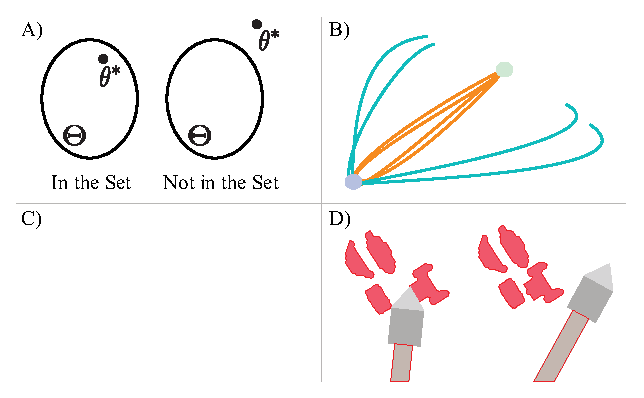
\includegraphics[width=0.5\textwidth]{f_figs/teaser.eps}
\caption{
    \footnotesize
A) An illustration of  the expert's policy, $\pi_{\theta^*}$ being contained in the robot's policy class $\Theta$. We argue that in the case on the right, passive LfD can be advantageous compare to adaptive. B) Samples taken from a robot trying to reach the green goal state. The adaptive approach(Teal) causes the robot to visit states the passive (Orange) does not need to. C) A person from our pilot study using an Xbox Controller to provide a demonstration to the robot on how to singulate an object from the pile. D) In the pilot study,  passive (left) always had visit the states the expert did, but adaptive (right) lead to states where the expert had to provide more complex commands such as teaching the robot to go backwards.}
\vspace*{-20pt}
\label{fig:teaserl}
\end{figure}

\mlnote{waiting on Anca for help on this paragraph}
 We tested the occurrence of  these problems via a pilot study with 10 roboticists at UC Berkeley, who were asked to use both DAgger and Passive Lfd to train a Zymark robot to singulate an object (or separate it from a pile). We observed a statistically significant gap in the average performance of the policies trained by the two approaches. In our  post analysis we examined how well people could match their controls in retro-active feedback compared to tele-operated. Furthermore, we examined a held out test set's surrogate loss to illustrate how well the policy learned is able to match the unseen data, which is related to how hard the demonstration can be to learn from. 


Additionally, we present three theoretical contributions. First, we show adaptive algorithms, despite having the same function class as the expert, on the expert's distribution, can with non-zero probability not recover the expert policy with infinite demonstration.However, passive LfD is able to do so. 


We furthermore contribute a new analysis for the error accumulation in passive LfD, that demonstrates for squared euclidean losses a tighter bound (in the time horizon of the task) than the rate suggested by Ross et al.~\cite{ross2010efficient}. We finally provide a data-dependent analysis of this rate for convex policy classes (i.e. linear SM, kernelized regression) using Rademacher Complexity, which shows that $T$ is not the only important parameter in analyzing policy error, but also size of policy class and number of demonstrations.

We  provide experiments in a gridworld domain with over 100 randomly generated environments demonstrating the effect of growing the robot's policy function class size. Result suggests that the performance difference, in terms of cumulative reward, between adaptive and passive is only seen when expert's policy is not contained in the set. We then illustrate a 2D point mass example, in which despite having the same function class as the expert, adaptivity fails to converge to the expert's policy. Finally, we test both DAgger and passive Lfd for learning a visuo-motor neural network policy for singulating objects from a pile on a Zymark Robot platform across 10 human subjects. We found the passive LfD is able to achieve a $21 \%$ increase in the probability of success with the same amount of data.




\section{Related Work}
Below we summarize related work in passive and adaptive LfD and their theoretical insights. \mlnote{Still working on this section}

\noindent \textbf {Passive LfD}
Pormeleau et al. used passive Lfd to train a neural network to drive a car on the highway via demonstrations provided by an expert. To reduce the number of demonstrations needed to perform a task, they synthetically generated  images of the road and subsequent labels~\cite{pomerleau1989alvinn}. A similar idea, was recently proposed by ~\cite{NVIDEA}, but used a convolutional neural architecture. 

Ross et al. examined the passive Lfd in a theoretical setting and derived that in the worst case the error from this approach can go quadratic in the time  horizon, $T$~\cite{ross2010efficient}. The intuition behind this analysis is that if the distribution induced by the robot's policy is different than the expert's, the robot could incur maximum error. 

In our analysis, we show that a rate of $T\sqrt{T}$ is achievable. However in contrast to Ross et al,  we also show how function class complexity and the number of demonstrations effect this bound. Data dependent results can help provide better insight into the error incurred in the finite sample domains. 

\noindent \textbf{Adaptive LfD}
Adaptive LfD has recently been used in numerous examples of model-free learning from high dimensional state representations, such as images. Successful robotic examples of adaptive LfD with an expert  include flying a quad-copter through a forest where the input is only image data taken from an on board sensor~\cite{ross2013learning}.

 Recently, Laskey et al. applied adaptive LfD to manipulation tasks such as surgical needle insertion \cite{laskeyshiv} and robotic de-cluttering, where a robot is given image data of a table with a variety of objects on it and must learn to push the obstacle objects aside to grasp a goal \cite{laskeyrobot}. Other successful examples have been teaching a robotic wheelchair to navigate to goal positions in the presence of obstacles and teaching a robot to follow verbal instructions to navigate across an office building \cite{kim2013maximum, duvallet2013imitation}. 

Algorithmic extensions to adaptive LfD have also been recently made, such as  forcing the expert to provide controls more similar to the robot's policy which allows for easier to learn policies~\cite{he2012imitation}. Furthermore, Kim et al. proposed to only query the expert in states that the robot is uncertain~\cite{kim2013maximum} and Laskey et al. extended this to high dimensional states~\cite{laskeyshiv}. Finally, Laskey et al. looked at using a hierarchy (in terms of quality) of experts to reduce burden on the expert supervisor~\cite{laskeyrobot}.

All these approaches build theoretically upon the online optimization analysis that Ross et al. proposed~\cite{ross2010reduction}. In online optimization an adversary presents a learner's policy with some cost function and the learner then chooses an action and receives a loss. In the LfD context, the learner chooses a policy and the adversary always select the expected disagreement with respect to the expert on the distribution induced by the policy~\cite{shalev2011online}. DAgger specifically can be modeled as a Follow The Leader algorithm, because it picks the best policy over all previous seen demonstrations~\cite{ross2010reduction}.

In the online optimization algorithm a bound for the error on the robot's policy can be obtained that is linear in $T$ for stongly convex losses (i.e. heavily regularized linear or kernelized regression). However as we show the regret bound does not imply convergence to the expert is possible, even when the robot's function class contains the expected expert's policy. 


\section{Problem Statement and Background}\label{sec:PS}
The goal of this work is to learn a policy that matches that of the expert on a specified task that demonstrations are collected on. 

\noindent\textbf{Modeling Choices and Assumptions}  We model the system dynamics as Markovian, stochastic, and stationary. Stationary dynamics occur when, given a state and a control, the probability of the next state does not change over time. 

We model the initial state as sampled from a distribution over the state space.
We assume a known state space and set of controls. We also assume access to a robot or simulator, such that we  can sample from the state sequences induced by a sequence of controls.   Lastly, we assume access to a expert who can, given a state, provide a control signal label. We additionally assume the expert can be noisy and imperfect, noting that the robot cannot surpass the performance level of the expert. 



\noindent\textbf{Policies and State Densities.}
Following conventions from control theory, we denote by $\mathcal{X}$ the set consisting of observable states for a robot task, consisting, for example, of 
high-dimensional vectors corresponding to images from a camera, or robot joint angles and object poses in the environment.
We furthermore consider a set $\mathcal{U}$ of allowable control inputs for the robot, which can be discrete or
continuous. We model dynamics as Markovian, such that the probability of state $\mathbf{x_{t+1}}\in
\mathcal{X}$ can be determined from the previous state $\mathbf{x}_t\in\mathcal{X}$ and control input $\mathbf{u}_t\in
\mathcal{U}$: 
$$p(\bx_{t+1}|\bu_{t},\bx_{t}, \ldots, \bu_{0}, \bx_{0})=p(\bx_{t+1}|\bu_{t}, \bx_t)$$
We assume a probability density over initial states $p(\bx_0)$. The environment of a task is thus defined as a specific instance of a control and stat space, initial state distribution and dynamics. 


%We denote the probability density over the initial state also by $p:\mathcal{X}\to \mathbb{R}$. 

A trajectory $\hat{\tau}$ is a finite sequence of $T+1$ pairs of states visited and corresponding
control inputs at these states, $\hat{\tau} = (\mathbf{x}_0,\mathbf{u}_0, ...., \mathbf{x}_T,\mathbf{u}_T)$, where $\bx_t\in \mathcal{X}$
and $\bu_t\in \mathcal{U}$ for $t\in \{0, \ldots, T\}$ and some $T\in \mathbb{N}$.  
For a given trajectory $\hat{\tau}$ as above, we denote by ${\tau}$ the corresponding trajectory in state space,
${\tau} = (\bx_0,....,\bx_T)$.


A policy is a measurable function $\pi: \mathcal{X} \to \mathcal{U}$ from states to control inputs. 
We consider a set of policies $\pi_{\theta}:\mathcal{X}\to \mathcal{U}$ parameterized by some $\theta\in \Theta$. Any such policy $\pi_{\theta}$ in an environment with probabilistic initial state density and Markovian dynamics
induces a density on probability measure over the set of  trajectories of length $T+1$: $$p(\tau | \theta)=
p(\bx_0)\prod_{i=0}^{T-1}p(\bx_{t+1}|\bu_t,\bx_t)p(\bu_t|\bx_t,\theta)$$


While we do not assume knowledge of the distributions corresponding to: $p(\bx_{t+1}|\bx_t,\bu_t)$, $p(\bx_0)$ or $p(\bx_t|
\theta)$, we assume that we have a stochastic real robot or a simulator such that for any state
$\bx_t$ and control $\bu_t$, we can sample the $\bx_{t+1}$ from the density $p(\bx_{t+1}|\bu_t,\bx_t)$. 
Therefore, when 'rolling out' trajectories under a policy
$\pi_{\theta}$, we utilize the robot or a simulator to sample the resulting stochastic trajectories rather than
estimating $p(\bx|\theta)$ itself.


\noindent\textbf{Objective.} The objective of  policy learning is to find a policy that minimizes some known cost function $C(\hat{\tau}) = \sum^T_{t=1} c(\bx_t,\bu_t)$ of a trajectory $\hat{\tau}$. The cost $c:\mathcal{X}\times \mathcal{U}\to \mathbb{R}$ is typically user defined and task specific. 
For example, in the task of inserting a peg into a hole, a function on distance between the peg's current and desired final state is used \cite{levine2015end}.  


In our problem, we do not have access to the cost function itself. Instead, we only have access to 
a expert, $\pi_{\theta^*}$, where $\theta^*$ may not be contained in $\Theta$. A expert is chosen that can achieve a desired level of performance on the task. The expert provides the robot an initial set
of $N$   demonstration trajectories $\lbrace \tilde{\tau}^1,...,\tilde{\tau}^N \rbrace$. 
which are the result of the expert applying this policy. This induces a training data set $\mathcal{D}$ of all state-control input pairs from the demonstrated trajectories.

We are interested in determining what parameter $\theta$ generates the sample demonstrations from the expert's policy. 

\noindent \textbf{Passive LfD} Passive Lfd frames this  question as maximizing the conditional likelihood of the sample demonstrations conditioned on a given parameter $\theta$. 

$$\underset{\theta}{\mbox{max}} \prod^N_{n=1} p(\bx_{0,n}) \prod^T_{t=1} p(\bx_{t+1,n}|\bx_{t,n},\bu_{t,n})p(\bu_{t,n}|\bx_{t,n},\theta)$$

In solving this optimization it is common to optimize the conditional log-likelihood, which maintains the same solution but breaks up the product terms into sums. 

\begin{equation}\label{eq:m_likeli_obj}
\underset{\theta}{\mbox{max}} \sum^N_{n=1}\sum^T_{t=1}\mbox{log }p(\bu_{t,n}|\bx_{t,n},\theta)
\end{equation}


We note that the dynamics and initial state distributions are dropped in this objective because they are conditionally independent of $\theta$, once the controls are observed. 

 Traditionally maximizing the probability of a given control observed from the expert, has been viewed as minimization of a surrogate loss to denote a difference between the true cost function~\cite{ross2010reduction,ross2010efficient}. We will refer the to function $l : \mathcal{U} \times \mathcal{U} \rightarrow \mathbb{R}$ as the surrogate loss through out this paper. The surrogate loss can either be an indicator function as in classification or a continuous measure on the sufficient statistics of $p(\bu|\bx,\theta)$.  This rewrites the objective as follows: 

\begin{equation}\label{eq:main_obj}
\theta^N = \underset{\theta}{\mbox{argmin}} \sum^N_{n=1}\sum^T_{t=1} l(\bu_{n,t}, \pi_{\theta} (\bx_{n,t})).
\end{equation}


\noindent \textbf{Adaptive LfD} Due to model mismatch (e.g. not being realizable), or a limited amount of data, solving Eq. \ref{eq:main_obj} may not lead to $\theta^N \neq \theta^*$.  Thus, leading to a mismeasure in the distribution trained on and tested on, since the robot visits states from the distribution $p(\tau|\theta^N)$ and not the expert's, $p(\tau|\theta^*)$.  Prior work has proposed an adaptive solution ~\cite{ross2010reduction} that attempts to solve this problem by aggregating data on the distribution induced by the current robot's policy.

Instead of  minimizing the surrogate loss, in Eq. \ref{eq:main_obj},  DAgger attempts to find the distribution the final policy will converge to, reducing surrogate loss in places the robot is likely to visit.
DAgger~\cite{ross2010reduction} attempts this by iterating two steps: 1)
computing the policy parameter $\theta$ using the training data $\mathcal{D}$ thus far, and 2) by executing the policy
induced by the current $\theta$, and asking for labels for the encountered states. 
 
\subsubsection{Step 1}
The first step of any iteration $k$ is to compute a $\hat{\theta}_k$ that minimizes surrogate loss on the current dataset $\mathcal{D}_k=\{(x_i,u_i)|i\in\{1,\ldots,N\}\}$ of demonstrated state-control pairs (initially just the set $\mathcal{D}$ of initial trajectory demonstrations):

 \vspace{-1ex}
\begin{align}\label{eq:super_objj}
\theta_{k} = \underset{\theta}{\argmin} \: \sum_{i=1}^{N} \sum_{t=1}^T  l(\pi_{\theta}(\bx_{i,t}),\bu_{i,t}).
\end{align}

This can be observed as minimizing the empirical risk on the aggregate dataset of all examples seen so far~\cite{scholkopf2002learning}.  Note that equal weight is given to each example regardless of how likely they are under the current policy.
 

 \subsubsection{Step 2}
The second step at iteration $k$, DAgger rolls out the current policy, $\pi_{\theta_{k}}$, to sample states that are likely under $p(\tau|\theta_{k})$.  For every state visited, DAgger requests the expert to provide the appropriate control/label. Formally, for a given sampled trajectory  $\hat{\tau} = (\bx_0,\bu_0,...,\bx_T,\bu_T )$, the expert provides labels $\tilde{\bu}_t$, where $\tilde{\bu}_t \sim \tilde{\pi}(\bx_t) + \epsilon$, where $\epsilon$ is a  zero mean noise term, for $t\in \{0, \ldots, T\}$.
The states and labeled controls are then aggregated into the next data set of demonstrations $\mathcal{D}_{k+1}$:
$$D_{k+1}=\mathcal{D}_k \cup \{(\bx_t,\tilde{\bu_t})|t\in\{0,\ldots,T\}\} $$

Steps 1 and 2 are repeated for $K$ iterations or until the robot has achieved sufficient performance on the
task\footnote{In the original DAgger the policy rollout was stochastically mixed with the expert, thus with
    probability $\beta$ it would either take the expert's action or the robots. The use of this stochastically mix
    policy was for theoretical analysis and in practice, it was recommended to set $\beta = 0$ to avoid biasing the
sampling~\cite{NIPS2014_5421,ross2010reduction}}.


 

\section{Theoretical Analysis}
In this section we will first show how adaptive algorithms can cause the robot's policy to not converge. Then we present a new analysis for the accumulation in error for  passive LfD.  Finally, we use Rademacher Complexity to illustrate how function class and number of demonstrations affect the worst case error. 

For this section are interested in the total cost along a trajectory with respect to a policy, $\pi_{\theta}$, which is defined as $J(\theta) = \sum^T_{t=1} l(\pi_{\theta}(\bx_{t}),\pi_{\theta^*}(\bx_{t}))$. 

\subsection{Algorithm Convergence}
\mlnote{We are working on formalizing this section more}
Convergence of an LfD algorithm can be defined in a number of ways, for example one way could be the element-wise condition $\theta^* = \hat{\theta}$. However, this is potentially a stronger condition than required for the performance of a robot to match that of an expert.  This is because the robot only needs to match the expert on the distribution induced by the expert (i.e. if the expert never visits a state the robot should not be forced to match the expert there). 

An algorithm converges if
$$\underset{n \rightarrow \infty}{\text{limit }} E_{p(\tau|\theta^*)}J(\theta^N)  = E_{p(\tau|\theta^*)}J(\theta^*) $$
\noindent where $\theta^N$ is the result of running an algorithm on $N$ datapoints.

This statement implies that the policy achieves the same surrogate loss of the expert's policy on the distribution of states the expert visits. Thus, agrees with the expert in all states the expert would visit.  The function class $\Theta$ and choice of learning algorithm that achieves this condition will be defined as consistent~\cite{vapnik1992principles}.

We will now show that it is possible for a given policy class, $\Theta$, to achieve have this condition when using passive LfD, but fail to when using an adaptive LfD. \\
Let $\theta_{p}^M$ be the result of running passive LfD on $M$ trajectory samples from the supervisor.
Let $\theta_{d}^N$ be the result of running DAgger for $N$ iterations.

\begin{figure}
\centering
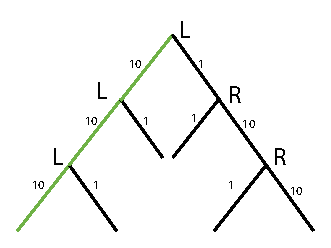
\includegraphics{f_figs/counter_exmp.eps}
\caption{
    \footnotesize
A binary decision tree, where a robot is being taught by a expert to descend down and achieve maximum cumulative reward, which is shown via the numbers on each branch. Each node has the action the expert would select, either left or right, $\lbrace L, R \rbrace$. The optimal policy, colored in green, is to select left, $L$, at each node.}
\vspace*{-20pt}
\label{fig:c_ex}
\end{figure}

\jmnote{Need to get the notation consistent}
\jmnote{Should change rewards to costs in examples to be consistent with definitions}
\jmnote{Might want to make a, explicit statement in the theorem about the policy being realizable to make things stronger although it's already in there technically}
\begin{theorem}
There exists an environment and policy class $\Theta$ such that:
\begin{align*}
	\underset{N \rightarrow \infty}{\text{lim }} E_{p(\tau \mid \theta_{d}^N) } J(\theta_{d}^N) &> E_{p(\tau \mid \theta^*)} J(\theta^*) \\
	\underset{M \rightarrow \infty}{\text{lim }} E_{p(\tau \mid \theta_{p}^M) } J(\theta_{p}^M) &= E_{p(\tau \mid \theta^*)} J(\theta^*)
\end{align*} 
\noindent In other words, DAgger may fail to converge in cases where passive LfD matches the expert exactly.
\end{theorem}

\begin{proof}
Consider an environment with a deterministic initial state at the root of a binary tree of depth 3 with deterministic dynamics and rewards illustrated in Fig. \ref{fig:c_ex}.
Let $T = 3$ and consider the 0-1 surrogate loss $\ell$.
The optimal policy is to choose to go left at the initial state at every branch on the left of the tree and right at every branch on the right of the tree.
This incurs cost $E_{p(\tau \mid \theta^*)} C(\tau) = 21$ and expected surrogate loss $E_{p(\tau \mid \theta^*)} J(\theta^*) = 0$.

Let the policy class for DAgger and supervised learning be the set of policies $\Theta = \{L, R\}$.
Let $\mD_K$ be a set of $K * T$ states generated by the algorithm, and let $a = \sum_{x \in \mD_K} \mathbf{1}(\pi^*(x) = R)$ and $b = \sum_{x \in \mD_K} \mathbf{1}(\pi^*(x) = L)$ count the number of states in which the expert chose right and left, respectively, where $\mathbf{1}$ is the indicator function. 
Then the policy produced by either algorithm is $\pi_{\hat{\theta}}(x) = \hat{\theta}$ for all states $x$, where
\vspace{-2ex}
\begin{align*}
	\hat{\theta} = \underset{\theta \in \Theta}{\text{argmin }} \sum_{k=0}^K \sum_{t=0}^T \ell(\pi_{\theta}(x_{k,t}), \pi_{\theta^*}(x_{k,t})) = \left\{ \begin{array}{cc} R & a \geq b \\ L & a < b \end{array} \right.
\end{align*}
\noindent In other words, the optimal policy is to choose the action that the expert chooses most frequently in the dataset.

For supervised learning, the dataset $\mD_K$ consists of $K * T$ left labels because the dynamics and initial state are deterministic.
Therefore for any $M > 0$ supervised learning chooses $\theta_{p}^M = L$ which has surrogate loss $E_{p(\tau \mid \theta_{p}^M)} J(\theta_{p}^M) = 0$.

Let DAgger be initialized with $\theta_d^0 = R$, and without loss of generality assume DAgger collects one trajectory per demonstration.
Then on iteration $N=1$, DAgger goes to the right three times and collects expert labels $\{L, R, R\}$, leading to policy $\theta_{d}^1 = R$.
Furthermore, if $\theta_{d}^K = R$ then the next iteration collects $\{L, R, R\}$ and the dataset $\mD_{K+1}$ maintains two-thirds right labels, so $\theta_{d}^{K+1} = R$.
Therefore by induction $\theta_{d}^{N} = R$ for all $N > 0$, which incurs surrogate loss $E_{p(\tau \mid \theta_{p}^N)} J(\theta_{p}^N) = (1 / 3) N T > E_{p(\tau \mid \theta_{p}^M)} J(\theta_{p}^M)$.
We also note that the cost incurred is suboptimal: $E_{p(\tau \mid \theta_{p}^N)} C(\tau) = 30$.
\end{proof}

It is interesting to note that this theorem does not contradict the original theoretical anlysis of Ross et al. ~\cite{ross2010reduction}. In their analysis, DAgger is modeled as a  an online optimization problem~\cite{ross2010reduction}.  In online optimization a learner plays a game where at each iteration, it chooses a policy and receives a loss from an adversary.  In the LfD setting, the learner is the robot's policy and the adversary would be the loss on the distribution of states induced by the policy $E_{p(\tau|\theta)} J(\theta)$~\cite{shalev2011online}.

DAgger in this context is known as a Follow the Leader (FTL) algorithm. In FTL, the best policy is chosen on all previous seen losses, or the aggregate dataset in the LfD context. Their analysis shows that under the condition when the surrogate loss, $l$, is strongly convex with respect to $\theta$, their policy has a regret that converges to the best the policy could have done on all previous seen losses $\underset{\theta}{\min} \sum_{k=1}^K E_{p(\tau|\hat{\theta}_k)}J(\hat{\theta}_k)$. 

A bound in regret though though does not necessarily imply the robot will be able to generalize to the unseen data nor match the expert. It instead says the robot's error is bounded by the best it could have done in hindsight, which may be arbitrarily bad as our tree example suggests. 

We acknowledge that these  problem can be overcome by increasing the robot policy's function class. However, a larger function class could result in more data needed to learn the policy than the passive LfD and be more susceptible to noise~\cite{kakade2009generalization}.

\subsection{Bound on Error for Passive Lfd}
In the passive LfD setting a robot is trained on the states visited by the expert. However, at run time it can encounter a different distribution of states due to not perfectly matching the expert's policy. Ross et al. showed that given a time horizon, $T$, the worst case error scales quadritically (i.e. $O(T^2E_{p(\bx|\theta^*)} l(\theta^N)$) when executing the robot's policy~\cite{ross2010efficient}. Note according to the notation of Ross et al., $TE_{p(\bx|\theta^*)} l(\theta^N) = E_{p(\tau|\theta^*)} J(\theta^N)$. We present a new analysis for a specific class of policies defined below that shows a rate of $O(T\sqrt{TE_{p(\bx|\theta^*)} l(\theta^N)}$, which suggests a tamer rate in the time horizon. 

 Define the surrogate loss as the squared euclidean norm, or $l(\pi_{\theta}(\bx),\pi_{\theta^*}(\bx)) = ||\pi_{\theta}(\bx_{i,t}) - \pi_{\theta^*}(\bx_{i,t})||_2$.We assume that the controls are be bounded and thus can be normalized such that the $l \in [0,1]$.  We are interested in the situation where the expert and robot policy are stochastic with a Normal Distribution (i.e. $p(\bu|\pi_{\theta}(\bx)) = \mathcal{N}(\pi_\theta(\bx),\sigma I)$. A stochastic policy with a normal distribution is a common assumption for learned robotic policy ~\cite{levine2015end}. 
 

\begin{theorem}
Given a policy $\pi_{\theta^N}$, the following is true 
$$E_{p(\tau|\theta^n)} J(\theta^N) \leq \sqrt{T\frac{1}{4\sigma}E_{p(\tau|\theta^*)} J(\theta^N)}+E_{p(\tau|\theta^*)} J(\theta^N)$$\\
\end{theorem}
\begin{proof}
For convenience we will write $E_{p(\tau|\theta)} = E_{\theta}$ and $l(\theta,\bx) = l(\theta)$. 

\begin{align}
&E_{\theta^N} J(\theta^N) - E_{\theta^*} J(\theta^N) \\
&= T(\frac{1}{T}E_{\theta^N} J(\theta^N) -\frac{1}{T}E_{\theta^*} J(\theta^N)\\
&\leq  T| | p(\tau|\theta^N) - p(\tau|\theta^*)||_{TV}\\
&\leq T\sqrt{\frac{1}{2} D_{KL}(p(\tau|\theta^*),p(\tau|\theta^N))}
\end{align}

 Line 6 leverages the fact that the worst case loss is bounded by $1$ and the definition of Total Variational distance. Line 7 uses Pinsker's inequality. 


\begin{align}
&= T\sqrt{\frac{1}{2} E_{p(\theta^*)} \mbox{log} \frac{p(\tau|\theta^*)}{p(\tau|\theta^N)}}\\
&= T\sqrt{\frac{1}{2} E_{p(\theta^*)} \sum^T_{t=1}\mbox{log} \frac{p(\bu_t|\bx_t,\theta^*)}{p(\bu_t|\bx_t,\theta^N)}}\\
&= T\sqrt{\frac{1}{4\sigma} E_{p(\theta^*)} \sum^T_{t=1} ||\bu_t- \pi_{\theta^N}(\bx_t)||_2^2 - ||\bu_t- \pi_{\theta^*}(\bx_t)||_2^2}\\
&\leq T\sqrt{\frac{1}{4\sigma} E_{p(\theta^*)} \sum^T_{t=1}  ||\pi_{\theta^*}(\bx_t) - \pi_{\theta^N}(\bx_t)||_2^2}\\
&= T\sqrt{\frac{1}{4\sigma} E_{p(\theta^*)} J(\theta^N)}\\
&= T\sqrt{T \frac{1}{4\sigma} E_{p(\bx|\theta^*)} l(\theta^N)}
\end{align}

Line 8,9 and 10 apply the definition of the KL-divergence, the markov chain and the normal distribution over $p(\bu_t|\bx_t,\theta)$. Line 11 applies the triangle inequality to upperbound by the defined surrogate loss. Line 12 applies the assumed definition of $J(\theta)$. Line 13 uses Ross et al. notation. 

The intuition behind these steps is that difference between  the two distribution can be controlled via the surrogate loss on the expected expert. Thus, illustrating the closer the robot's policy matches the expert's policy on the expert's distribution, the smaller the total variational difference between the resulting two distributions will be. 
\end{proof}
  
It is important to note that our bound can be larger than the original analysis provided by Ross et al. when  $E_{p(\bx|\theta^*)} l(\theta^N)$ is very small. However, when not enough demonstrations have been collected or model error exists $E_{p(\bx|\theta^*)} l(\theta^N)$ could be quite large. Thus, suggesting that passive Lfd has more robustness than originally thought. 

\subsection{Finite Sample Analysis}
The above analysis demonstrates how the constant $T$ affects the bound in error. However, it is important to note that this is not the only variable that plays a role in performance. The size of the function class and number of demonstrations needed are are also important. 

Understanding how much data is needed to learn a function, is a well studied problem known as sample complexity analysis~\cite{anthony2009neural}. In this literature they use different metrics to describe the complexity of a function class and show rates on which a given function class would converge to the real solution. We refer the reader to \cite{vapnik2013nature}, for a review of such topics. 

An example of such results though is the following.  If we are interested in the total cost along a trajectory with respect to a policy, $\pi_{\theta}$, which is defined as $J(\theta) = \sum^T_{t=1} l(\pi_{\theta}(\bx_{t}),\pi_{\theta^*}(\bx_{t}))$.  If we assume the surrogate loss $l$ is convex with respect to $\theta$ and bounded between $[0,1]$, then if $\theta \in \Theta$. \\

\begin{theorem}\label{thm:sup}
For a policy, $\theta^N$ found via passive LfD, from $N$ trajectories collected from the expert the following is true with probability at least $1- 2\mbox{exp} (-N\delta^2/8)$

$$E_{p(\tau|\theta^*)} J(\theta^N)\leq T( 2R_{\Theta}(N) + \delta+ O(\frac{1}{\sqrt{N}})) + E_{p(\tau|\theta^*)} J(\theta^*)$$\\

\end{theorem}

The proof for this analysis can be found in Sec. 3 in Tewari et al.~\cite{tewari13learning}. In this result, $R_{\Theta}(N)$ corresponds to the Rademacher complexity of the given function class $\Theta$ for $N$ samples.
The Rademacher complexity is a measure of much a function can fit to random noise.
Intuitively, more complex function classes may fit noise better, leading to slower rates of convergence.
The Rademacher Complexity for bounded linear functions and kernel regressors over bounded domains is $O (\frac{1}{\sqrt{N}})$ ~\cite{bartlett2002rademacher, kakade2009complexity}.
For decision trees with linear decision functions, the Rademacher Complexity is $O (\frac{1}{\sqrt{N}} + \frac{\log(N)}{N}$ ~\cite{bartlett2002rademacher}.

\jmnote{I'd vote to remove the below, it's hard to relate the terms to T dues to unknown constant factors}
Thus if your expert's policy is only a linear function, you may find the Rademacher term is small enough that $T$ is the dominant factor. However, if you are trying to learn a highly non-linear function, the Rademacher complexity could be much larger than $T$~\cite{vapnik2013nature} Thus, suggesting that only examining $T$ in the analysis can be misleading. 


\section{Experiments}

\begin{figure*}
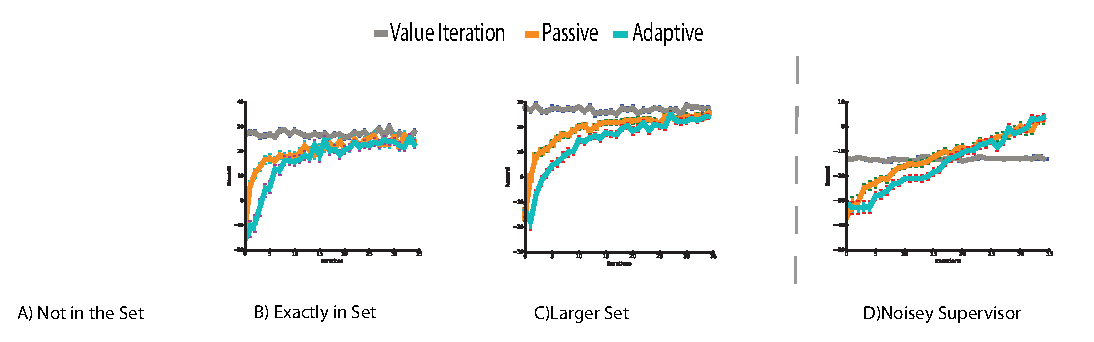
\includegraphics{f_figs/var_grid.eps}
\caption{
    \footnotesize
Shown above is the normalized performance with respect to the expected expert, where $1.0$ indicates matching the expected expert's reward. The plots are averaged over 100 randomly generated 2D gridworld environments,  where the robot is taught to avoid penalty states and reach a goal state. A) Examines when the robot's policy class (i.e. Linear SVM) is not able to learn the expert's, which results in adaptivity leading to better performance. Condition B examines a larger robot policy class (i.e. Decision Trees) that contains the expected expert,and demonstrates negligible difference between adaptive and passive LfD.  to represent the expert.  Finally, Condition C examines when the expert has noise added to the controls labels, this leads to more data being needed to converge to the expected expert, but the difference between passive and adaptive is still negligible.   }
\vspace*{-20pt}
\label{fig:var}
\end{figure*}

We provide experiments in a simulated GridWorld environment, which allows for us to vary the robot's policy class over a large number of randomly generated enviroments. Then we examine a linear dynamical system, which is used to show a limitation the ability of adaptive algorithms to converge. Finally, we perform human trials on 10 participants, who try to teach a robot how to singulate, or separate an object from a pile. 

\subsection{Varying Function Class}\label{sec:gdw}
In this experiment, we hypothesize that the performance gap of adaptive LfD diminishes as the the robot's policy class is increased. In a simulated GridWorld, we have a point robot that is trying to reach a goal state, at which it receives $+10$ reward. The robot receives $-10$ reward if it touches a penalty state, as shown in Fig. \ref{fig:grid_world}. The robot also receives a $-0.02$ penalty for every blank state. The robot has a state space of $(x,y)$ coordinates and a set of actions consisting of $\lbrace$LEFT,RIGHT,FORWARD,BACKWARD NONE$\rbrace$, where NONE indicates staying at the current stop. The grid size for the gridworld environment was $30 \times 30$ $20\%$ of randomly drawn states are marked as a penalty, while only one is a goal state. For the transition dynamics $p(\bx_{t+1}|\bx_{t},\bu_t)$, the robot goes to an adjacent state that does not necessarily correspond to the intended control with probability $0.2$.  The time horizon for the policy was $T=30$. 

We use Value Iteration to compute an optimal expert for our grid world domain. The optimal policy must learn to be robust to the noise in the dynamics, reach the goal state and then stay there. In all settings we provided the adaptive approach with one demonstration from the expert and then roll out its policy. 

Each plot shows the normalized performance where $1.0$ represents the expected performance of the value iteration expert. We run all trials over 100 randomly generated environments, which contain $X$ randomly selected penalty state and $1$ goal state. 


\noindent \textbf{Not in the Set} In Fig. \ref{fig:var} A, we show the case when the robot's policy class does not contain the expert's, we used a Linear SVM for the policy class representation, which is commonly used in ~\cite{ross2010efficient,ross2010reduction,ross2013learning} . As illustrated the Adaptive DAgger approach does better than the Passive approach, which is a common result in the literature~\cite{ross2010efficient,ross2010reduction}.


Similar to prior work passive LfD  with a Linear SVM does worse than DAgger, which iteratively determines the distribution it policy induces and minimize the expected risk on it. However, because the robot's policy class did not contain the expert's it was not able to perform as well as the value iteration expert. 

\noindent \textbf{In the Set}
We next consider the situation where the robot's policy class contains the expected expert. We used decision trees with a depth of $100$ to obtain a complex enough function class to achieve this. 

As shown in Fig. \ref{fig:var}, DAgger and passive LfD both converge to the expert, but at the same rate. Thu, suggesting that advantage of using DAgger diminishes once the expected expert is in the robot's policy class. We note that because the robot's policy class obtains the expert's convergance to the expert's performance is now obtained. 




\noindent \textbf{Noisy Expert}
We finally observe the effects of noise on the expert. Here we consider the case where noise is applied to observe label, thus the robot receive control labels that are $\bu = \pi_{\theta}(\bx) + \epsilon$,  where epsilon is an i.i.d distribution that selects a random control with probability $0.3$.

We use the  decision tree  of depth $100$ which due to its large function class is more susceptible to the noisy expert. We then compare the performance of passive versus adaptive LfD. As shown, both passive and adaptive are able to converge to the expected expert's normalized performance because they can average out the noise in the labels with enough data. Though it does take more data because passive LfD  and DAgger converge at a similar rate to the true expected expert. 




\subsection{Algorithmic Convergence }
In this experiment, we will demonstrate how adaptive techniques can fail to converge despite having the necessary function class to match the expert. 
We  consider the example where the robot needs to learn to get to a location in a 2D continuous world domain. The robot is represented as a point mass dynamics and the expert is computed using the infinite time horizon LQG, which results in a linear policy. 

The environment contains two sets of dynamics: 

$$x_{t+1} = A_1\bx_{t+1}+B_1\bu_t+w$$
$$x_{t+1} = A_2\bx_{t+1}+B_2\bu_t + w$$

where $w\sim \mathcal{N}(0,\sigma I)$. The dynamics for region B correspond to the controls being inverted for dynamics A. A target goal state and start state both lie in region A. 

The expert is a switching linear system, where each linear model is computed via the infinite horizon LQG for the specified dynamics. The robot's policy, $\pi_{\theta}$ is represented as a linear policy which is found via ridge regression.

We run passive Lfd and DAgger in this setting and plot the performance in Fig. \ref{fig:p_mass}. As shown, passive LfD is able to converge to the true expert's policy however the adaptivitiy of DAgger forces it to enter the region B of the work space and subsequently try to learn the two different experts. Thus, preventing it from converging. 

\begin{figure}
\centering
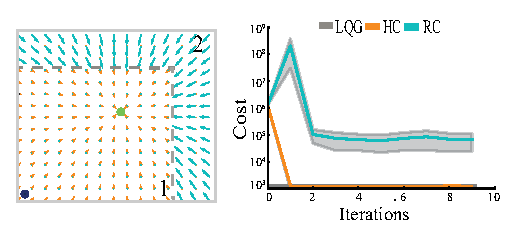
\includegraphics{f_figs/p_mass.eps}
\caption{
    \footnotesize
Left: A 2D workspace where a point mass robot is taught to go to the green circle starting from the blue circle. The world is divided into to two quadrants A and B, in B the controls are inverted in the dynamics thus resulting in $x=y$ and $y=x$. The expert is the infinite horizion LQG computed policy, which results in two different linear matrices in region A and B. Right: Illustrates how having a linear robot policy class can cause DAgger to fail  to converge due to it collecting data from region B.  }
\vspace*{-1pt}
\label{fig:p_mass}
\end{figure}

\subsection{Human Study for Planar Singulation}
We lastly perform a human study on a real robot, where people teach the robot to perform singulation task, or separate a object from a pile. Our hypothesis is that people will struggle providing retro-active feedback and cause the robot to try and learn more complex policies.  The objects used to form clutter are red extruded polygons.  For singulation task, we consider objects made of Medium Density Fiberboard with an average 4" diameter and 3" in height. 

The robot has a 2 dimensional internal state of base rotation and arm extension. The state space of the environment, $\mathcal{X}$, is captured by  an overhead Logitech C270 camera, which is positioned to capture the workspace that contains all cluttered objects and the robot arm. We use only the current image as state space, which captures positional information and a neural network architecture policy representation, the same as in~\cite{laskeyrobot}.

\begin{figure}
\centering
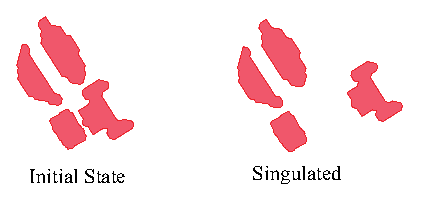
\includegraphics{f_figs/singulation.eps}
\caption{
    \footnotesize
Shown above is an example of an initial state (left) that the robot is presented with. It can vary in placement of the object in the pile, translation and rotation. A human is asked to singulate the object, which is to have the robot learn to push one object from the pile (right).  }

\label{fig:izzy_rw}
\end{figure}

The robot is commanded via position 
control with a  PID controller. Similar to \cite{laskeyshiv}, the controls, $\mathcal{U}$, to the robot are bounded changes in the internal state, which allows for us to easily register control signals to the demonstrations provided by experts as opposed to torque control. The control signals for each degree of freedom are continuous values with the following ranges: base rotation, $[-15^\circ,15^\circ]$, arm extension $[-1,1]$. The units are degrees for base rotation and centimeters for arm extension. 

During training and testing the initial state distribution $p(\bx_0)$ consists of sampling the relative pose of 4 objects from a distribution around their position in the pile and the pose of the pile as a whole. The pose of the pile is sampled from a Gaussian with variance \mlnote{get numbers}. Then using a virtual overlay,  a human is asked to place objects in their correct pose. 

The robot can be trained in either 2 ways DAgger or passive learning. In passive learning, the subject is asked to provide 60 demonstrations to the robot using an Xbox Controller. In active learning the user is first asked to provide 20 demonstrations via the Xbox Controller and then provides retro-active feedback for $K=2$ iterations of 20 demonstrations each. They used the same overlay technique as in ~\cite{laskeyrobot} to provide feedback. 

10 human subjects were selected who had a background in robotics research, but not in LfD. They were given a short demonstration of the learned robot policy and then asked to practice providing feedback through DAgger for 5 demonstrations and passive for 5 demonstrations. We then have each subject provide the first 20 demonstrations via passive feedback and then using counter-balancing to select whether they will perform passive or DAgger for the next 40 demonstrations.  

In Fig. \ref{fig:izzy_rw} , we show the average performance of the policies trained with DAgger and passive LfD. Each policy is evaluated on a hold out set of 30 initial states sampled from the same distribution as training. As shown, the policies learned with DAgger exhibit statistically significant worse performance than those with passive LfD. Thus, sugggesting that DAgger could perform worse than passive Lfd on a task with actual human supervision. 

\noindent \textbf{Post Analysis}
To better understand why DAgger performed worst than Passive LfD, we examined the surrogate loss on a test set of 10 randomly selected trajectories.  As shown in Table 1, we observed the average test error over the policies trained with 60 demonstrations in both degrees of freedom (i.e. forward and rotation) is statistically significant higher. While, this does not imply the policy was necessarily more complex, it does indicate that the DAgger policies on average had a harder time generalize to unseen labels in the dataset. 




\begin{table}[t]
\centering
\begin{tabular}{ R{1.75cm}||R{2.5cm}| R{2.5cm}}
 %\hline
 %\multicolumn{4}{|c|}{Sensitivity Analysis for Convergence to Best Grasp for Thompson sampling} \\
 %\hline 
 & \multicolumn{2}{c}{Surrogate Loss on Test Set} \\
 \hline
\specialcell{\bf Algorithm\\ \bf Type} & \specialcell{\bf Forward\\ \bf (mm)} & \specialcell{\bf Rotation \\ \bf (rad)} \\
 \hline
Passive LfD & $2.1\pm 0.2$ & $0.009 \pm 0.001$ \\
Adaptive LfD & $3.4 \pm 1.0$    & $0.014 \pm 0.003$ \\
 %\hline
\end{tabular}
   \caption { \footnotesize  Shown above is the average surrogate loss on a held out set of 10 demonstrations from the the total 60 demonstrations collected for each 10 demonstrators. The confidence intervals are standard error on the mean, which indicate Adaptive LfD obtains a statistically significant higher surrogate loss in both degrees of freedom, forward and rotation. 
   }
		\tablabel{opt-p-comparison}
\vspace*{-20pt}
\end{table}


We further tried to gain some insight into how well people provide retro-active feedback. We asked participants to tele-operate the robot five times and then provide retro-active feedback via the DAgger interface to try and match the controls given by tele-operation. The controls of the human tele-operation with those given by retroactive feedback. We compared the controls via first normalizing them between $[-1,1]$ based on their bounds an then used squared euclidean distance of the rotation and translation control. The same loss used in training of the policy. This measurement gives a  percentage difference between the human's tele-operation actions, and their retroactive feedback.

 We performed this experiment with five subjects, and observed an average normalized distance of $0.44$, or $44\%$ deviation. These results indicate a large  difference between the controls applied by retroactive feedback and those applied by the human performing tele-operation.
 
 Under the assumption that tele-operation was the correct action the expert wanted, this would suggest our retro-active feedback interface caused the intention to be loss. We acknowledge that this might be remedy by providing a more intuitive labeling interface, however an inherent problem may exists of the expert never observing how the world is affected by their control. 

\begin{figure}
\centering
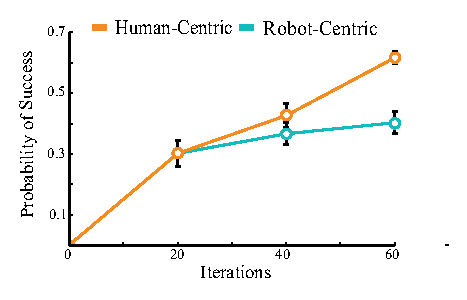
\includegraphics{f_figs/izzy_reward.eps}
\caption{
    \footnotesize
Shown is averaged success at the singulation task over the 10 human subjects. Each policy is evaulated 30 times on the a held out set of test configurations. The first 20 rollouts are from the expert rolling out there policy and the next 40 are collected via retro-active feedback for adaptive and tele-operated demonstrations for passive. Passive LfD shows a 20$\%$ improvement in success at the end. }
\vspace*{-20pt}
\label{fig:izzy_rw}
\end{figure}



\section{Conclusion and Future Work}
We thus conclude our analysis on the trade-offs between passive and adaptive Lfd approaches. We demonstrated that if a robot's function class contains the expected expert's policy, then the  performance difference between adaptive algorithms, such as DAgger,  and passive Lfd techniques can become negligible.  Furthermore, we also provided examples where adaptivity fails to converge despite being able to represent the expert. Thus illustrating a short-coming in the regret style analysis for DAgger. 

Our final experiment in having humans teach a robot to singulate objects suggest that adaptivity can lead to worse performance. Our post analysis seems to suggest that humans had a harder time providing retro-active feedback via a labeling interface. While, this may be overcome through a better labeling interface, an inherent problem persists in the inability of a human to observe how well their controls would have performed. 

Finally, we offered a new theoretical  way to analysis passive Lfd and demonstrate that the depedence on the time horizon constant, $T$, can be $O(T\sqrt{T})$ and not $O(T^2)$, a result that does not need the assumption of strongly convexity.  For convex loses, we are able to offer data-dependent sample complexity bounds that illustrate how the function class of the learning algorithm and number of demonstrations effect this bound on error. 

The data-dependent results demonstrate that in the worst-case a heavy tail could exits in terms of the number of demonstrations needed (i.e. a large number of demonstrations could be need). Thus, presenting a challenge in obtaining an industrial level of reliability in unstructured domains. However, in future work we are interested in examining ways around this limitation. Below are two possible ways:

\noindent \textbf{Active Learning} Uniform sampling from the initial state distribution $p(\bx_0)$, may not be an optimal approach to learning the expert's policy. In active learning, an algorithm would try to select more informative initial states for the robot to learn from. An example of this is the field of optimal design, where measurements are collected in a way to reduce variance in the label and lead to more robust data analysis. Extending this to LfD would be an interesting opportunity. 

\noindent \textbf{Synthetic Data Generation} Another approach to reduce data-dependence is to synthetically grow your dataset. For example, consider a robot learning how to grasp an isolated object  with image data as the state space. One could take the given image state and translate both the object and grasp label to create more demonstrations. A similar approach has been used recently in self-driving cars. However, a formal approach to checking when synthetic data generation is possible would be an exciting new direction. 

\bibliographystyle{IEEEtranS}
\bibliography{references}

\appendix
\subsection{Notation and Problem Statement}
Given a discrete-time stochastic dynamical system over the state-space $\mathcal{X}$ and control-space $\mathcal{U}$
\begin{equation}
x_{t+1} = f(x_t,u_t) + \epsilon_t~~x_0\sim p(x_0)~~\epsilon_t \sim \text{i.i.d}, \label{sde}
\end{equation}
both passive and adaptive LfD model the supervisor as a stochastic state-feedback control policy $\pi^*: \mathcal{X} \mapsto \mathcal{U}$:
\[
u_{t} \sim \pi^*(x_t).
\]
We assume that this distribution is parametric, parametrized by $\theta^* \in \Theta$, and where $\Theta$ denotes the parameter set over all possible policies--we will use $\pi_{\theta}$ to denote a given policy.  
Every policy parametrized by has a state distribution at time $t$:
\[x_t \sim \theta =  p(x_0) \prod^t_{i=1} p(x_{i+1}|x_{i},u_{i})p(u_i|x_i,\theta).\]
\sknote{how do you do retroactive feedback stochastically?}

Given independent and identically distributed episodic observations (each of a fixed-length $T$) of Equation \ref{sde}:
\[
D = \{d_1,...,d_N\}~~~~d_i = [(x_1,u_1),...,(x_T,u_T)],
\]
the LfD problem is to find a parametrized policy $\pi_{\theta}$ that minimizes the expected disagreement $\pi_{\theta^*}$ over $T$ time-steps of the system:
\begin{equation}
\min_{\theta \in \Theta} \sum_{t=0}^T \mathbf{E}_{x_t \sim \theta} [ \ell(\pi_{\theta}(x_t), \pi_{\theta^*}(x_t))]. \label{obj}
\end{equation}

\subsection{Empirical Risk Minimizer (Passive LfD)}
One approach to this problem is to find the $\hat{\theta}$ that minimizes the loss over each state seen in the demonstrations:
\[
\min_{\theta \in \Theta} \sum_{d=0}^N \sum_{t=0}^T \ell(\pi_{\theta}(x_{d,t}), u_{d,t}),
\]
and one can re-write this minimization problem as:
\begin{equation}
\hat{\theta} = \arg\min_{\theta \in \Theta} \sum_{d=0}^N  J(\theta),\label{erm}
\end{equation}
where $J(\theta) = \sum_{t=0}^T \ell(\pi_{\theta}(x_{d,t}), u_{d,t})$.
Equation \ref{erm} is called the empirical risk minimizer (ERM) as it estimates the true risk--the disagreement with the expected supervisor over the sample-space of demonstrations:
\[
\min_{\theta \in \Theta} \mathbf{E}_{d \sim D^\infty}  J(\theta).
\]
An important notion in ERM is consistency, i.e., $\hat{\theta} \rightarrow \theta^* \text{ a.s}$. This can be achieved for certain classes of functions via a uniform convergence argument \sknote{Someone who knows this advise--and replace consistency with whatever term you want}.
Our analysis assumes consistency and relaxing this assumption is a natural next step in future work.

\vspace{0.5em}\noindent \textbf{Remark: } Even with the fairly strong assumption of consistency, the LfD problem remains to be complex. The empirical risk minimization problem is measuring the expected risk over the distribution of states seen by the supervisor's policy. This is not quite the same as measuring the expected error over T time-steps of execution in Equation \ref{obj}. For any finite sample, the empirical risk minimizer will in general be $\hat{\theta} \ne \theta^*$, and the distribution of states visited by applying $\pi_{\hat{\theta}}$ might be different than the distribution of states visited by applying $\pi_{\theta^*}$.

\subsection{Follow-The-Leader (DAgger)}
To address the mismatch between supervisor and execution distributions, Ross et al. proposed an algorithm (DAgger) derived from online optimization rather than supervised learning. In online optimization, one usually considers a scenario where a sequence of data arrives in an unknown (and possible adversarial) stochastic process.
DAgger collects an initial set of $N'$ demonstrations, and computes the empirical risk minimizer $\hat{\theta}$.
Then, it executes this policy and collects samples of states visited by $\pi_{\hat{\theta}}$.
It appends these samples to the initial set of demonstrations and re-optimizes.
This approach is a form of online optimization called Follow-The-Leader, i.e., apply most successful, or ``leading'', parameter over the previous observations. 

\vspace{0.5em}\noindent \textbf{Remark: } Ross et al. proved a error bound with DAgger that showed error with DAgger is $\mathcal{O}(T\epsilon_n)$ where $\epsilon_n = \mathbf{E}_{d \sim D^\infty}  J(\hat{\theta})$. It is important to differentiate this bound from the hypothetical ``best policy in the class'', which would have $\epsilon = \mathbf{E}_{d \sim D^\infty}  J(\theta^*)$ and $\epsilon \le \epsilon_n$. In this sense, DAgger ensures that the error rate grows linearly with the best policy seen in the current dataset, but does not guarantee it will visit the same states (in distribution) as the supervisor as $N \rightarrow \infty$.







































\begin{defn}

\end{defn}

\subsection{Counterexample Proof Sketch}
Consider a robot learning to search down a tree with time horizon $T > 2$ to maximize cumulative reward as illustrated in Fig. \ref{fig:c_ex} with a policy that can choose to either always go left or always go right, $\Theta = \lbrace L,R \rbrace$.

The learning algorithm, which chooses how to update the policy is to choose the policy that satifies: 

$$\pi_{\theta} = \underset{\lbrace L,R \rbrace}{\mbox{argmin}} \sum^M_{m=0}\sum^T_{t=0} I(\pi_\theta(x_{m,t}),\tilde{\pi}(x_{m,t}))$$

It is straightforward to show that $\pi_{\theta}$ will always choose the majority of actions taken by the supervisor.

If passive LfD is applied to this situation, the expert will always chose left, $L$, and the robot will select this action resulting in perfect imitation. However, if DAgger is used and the robots initial policy is to go right, $\pi_{\theta_0} = R$.
Then for the first rollout the learner collects labels $\{L, R, ..., R\}$, and again chooses the policy $\pi_{\theta} = R$.
Furthermore, if on iteration $n$ $\pi_{\hat{\theta}_n} = R$ then the learner will again collect labels $\{L, R, ..., R\}$ and the aggregate dataset will still have a majority of $R$s.

Thus, convergence in regret is achievable because the best the robot could have done in hindsight would be to always choose $R$, but that does not result in a good policy. We note that if passive LfD was applied the robot would have chosen $L$ from the a single initial demonstration. 


\end{document}
Contact GitHub API Training Shop Blog About
© 2016 GitHub, Inc. Terms Privacy Security Status Help
